%% ============================================================
%%  §3 MLIR 的机制：层级如何变成一等对象
%% ============================================================

\section{机制：层级如何变成一等对象}
\label{sec:mechanisms}

上节说明每个系统都必须选层。MLIR 的特别之处不在于它"层更多"，而在于它\textbf{不把层的数量与
位置写进框架的前提}。本节只讨论撑起这一点的四个机制，不逐一介绍 MLIR 有哪些方言，那属于手册而不是论证。

\subsection{机制一：dialect 把"一层"搬到库边界}

一个 dialect 打包的是\textbf{一整套}设施：算子集合、类型与属性、验证规则，
以及可定制的打印/解析与规范化行为~\cite{mlir21}；这些由 ODS（Operation Definition
Specification）在构建期生成~\cite{mlirods}。

这一点常被低估。若"新增一层"意味着修改编译器内核（新增 IR 节点种类、改遍历与重写框架），
那么每加一层都要付内核级成本，层的数量必然稀缺；而 dialect 让这一整包东西成为
\textbf{可插拔的库单元}：新增一层不必改内核，只需链接一个库并注册。

\subsection{机制二：多级共存与部分下降}

MLIR 允许不同抽象高度的算子在同一个 module 里共存，且都是合法 IR。这不是实现细节，
而是"渐进下降"（progressive lowering）的前提：若层级不能共存，下降就只能整段一次性完成，
"分层"随即退化为"分阶段流水线"，复用单位也重新变成整条流水线。

图~\ref{fig:mixed-levels} 用真实语料把这一点变得可见。同一个文件里有两个函数：\texttt{@matmul}
用一次 \texttt{linalg.matmul} 表达整个矩阵乘，没有显式循环；\texttt{@matvec} 中同一计算已经
被显式化为 \texttt{scf.for} 循环加子算子 \texttt{linalg.matvec}。两者共存于同一 module 且都能
通过验证。由此可推出三件事：下降可以是\textbf{部分的}；层的边界是工程决策而非合法性约束；
因此最小复用单位可以是一条转换。

这条结论将在第~\ref{sec:evidence} 节被量化：正是因为它成立，"方言对"才能成为一个有意义的
成本计数单位。

\subsection{机制三：op interface 是可加性的技术根源}

这是本节最容易被写浅的一处。常见的表述是"interface 让不同 dialect 共享同一套操作"，
这既不准确也不够有力。真正起作用的是：\textbf{一条转换可以只依赖 interface 而不依赖具体方言，
因此不必为新方言重写}~\cite{mlirinterfaces}。

举例来说，tiling、fusion 这类变换只需要目标算子满足"可被切分"的接口约定，而不关心它是
\texttt{linalg.matmul} 还是某个厂商的私有算子。于是生态里新增一个方言时，已有变换往往可以
直接复用，这是 $N+M$ 而非 $N\times M$ 的技术根据。反过来，若没有 interface，每加一个方言
就要为每个变换写一遍适配，成本立刻退回乘法。

\subsection{机制四：conversion target 与 legality 让边界可声明}

层与层之间的边界在 MLIR 里是\textbf{可声明}的：conversion target 指明哪些
算子与类型在目标层合法，legality 规则据此判定"下降是否完成"，type converter 负责跨层的类型映射
~\cite{mlirconversion}。这使得"边界"本身成为可检验对象，可以问"这一步之后还有哪些非法算子
残留"，而不必靠人工判断"看起来下降完了"。

代价也是真实的：一条链上 pass 的顺序变得敏感，不完整的下降容易留下难以定位的残留。
这一点与 bufferization、shape 推断的困难一起，在第~\ref{sec:limitations} 节讨论。

\begin{figure}[t]
  \centering
  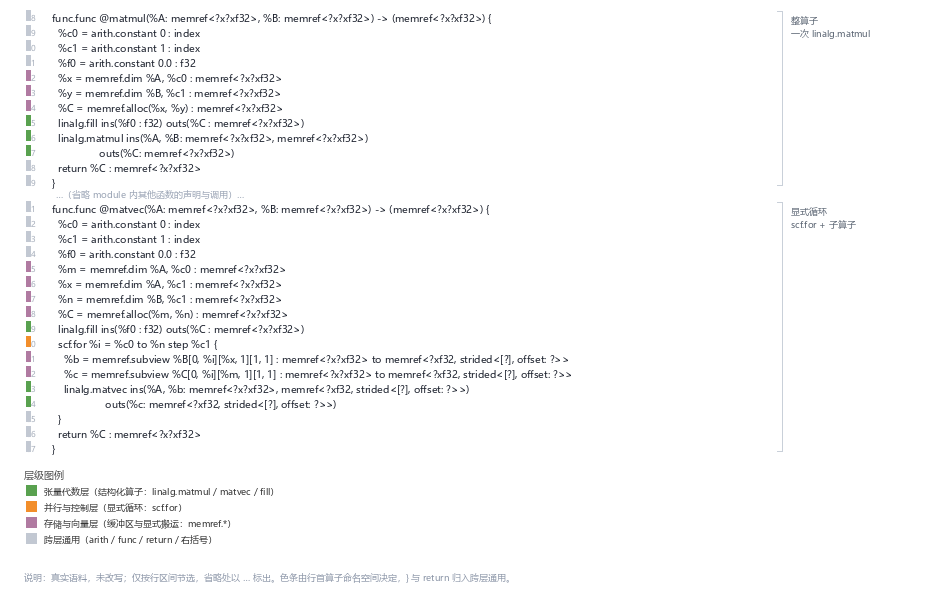
\includegraphics[width=\linewidth]{figures/fig_mixed_levels.png}
  \caption{同一 module 内的多级抽象共存。选自 \texttt{llvm-project@ba736172} 的
  \texttt{mlir/test/Integration/Dialect/Linalg/CPU/matmul-vs-matvec.mlir}，节选 29 行，未改写；
  左侧色条标出该行算子所属的抽象层。\texttt{@matmul} 以单个 \texttt{linalg.matmul} 表达
  整个矩阵乘；\texttt{@matvec} 中同一计算已被显式化为 \texttt{scf.for} 循环与子算子
  \texttt{linalg.matvec}。两者共存于同一 module，说明下降可以是部分的。}
  \Description{带层级色条的 MLIR 代码片段，两个函数分别使用整算子与显式循环}
  \label{fig:mixed-levels}
\end{figure}

\subsection{小结：机制的作用范围}

四个机制合起来说明：MLIR 不预设层数，其设施使层的划分可被协商。但这些机制只保证层可以被重新划定，
机制只保证"层可以被重新划定"，不保证"某一层会被多方采纳"。后者是生态问题，需要成本证据
（第~\ref{sec:evidence} 节）与治理证据（第~\ref{sec:contract} 节）才能回答。

第~\ref{sec:evidence} 节的实证正由这两个机制直接支撑：方言对之所以能作为可数的成本单位，
靠的是机制二（部分下降使单条转换有意义）与机制三（interface 使单条转换可跨方言复用）。
